For our solution we tried to do a 1:1 mapping directly from drawings to VHDL. This means that each ``box'' in our design
became a VHDL module. This lead to the three following files: ``Runner\_logic.vhd'',``Runner\_Registry.vhd'', ``Runner.vhd''.
The names of the files are corresponding to their function, except for ``Runner.vhd'' that maps the two other files together.\\
\subsection{Implementation}
When doing the physical design, we came across some issues that were handled by adding some extra components to out initial design. 
These changes can be seen in Figure \ref{fig:block_diagram_implementation}.
\begin{figure}[!htbp] 
	\centering 
        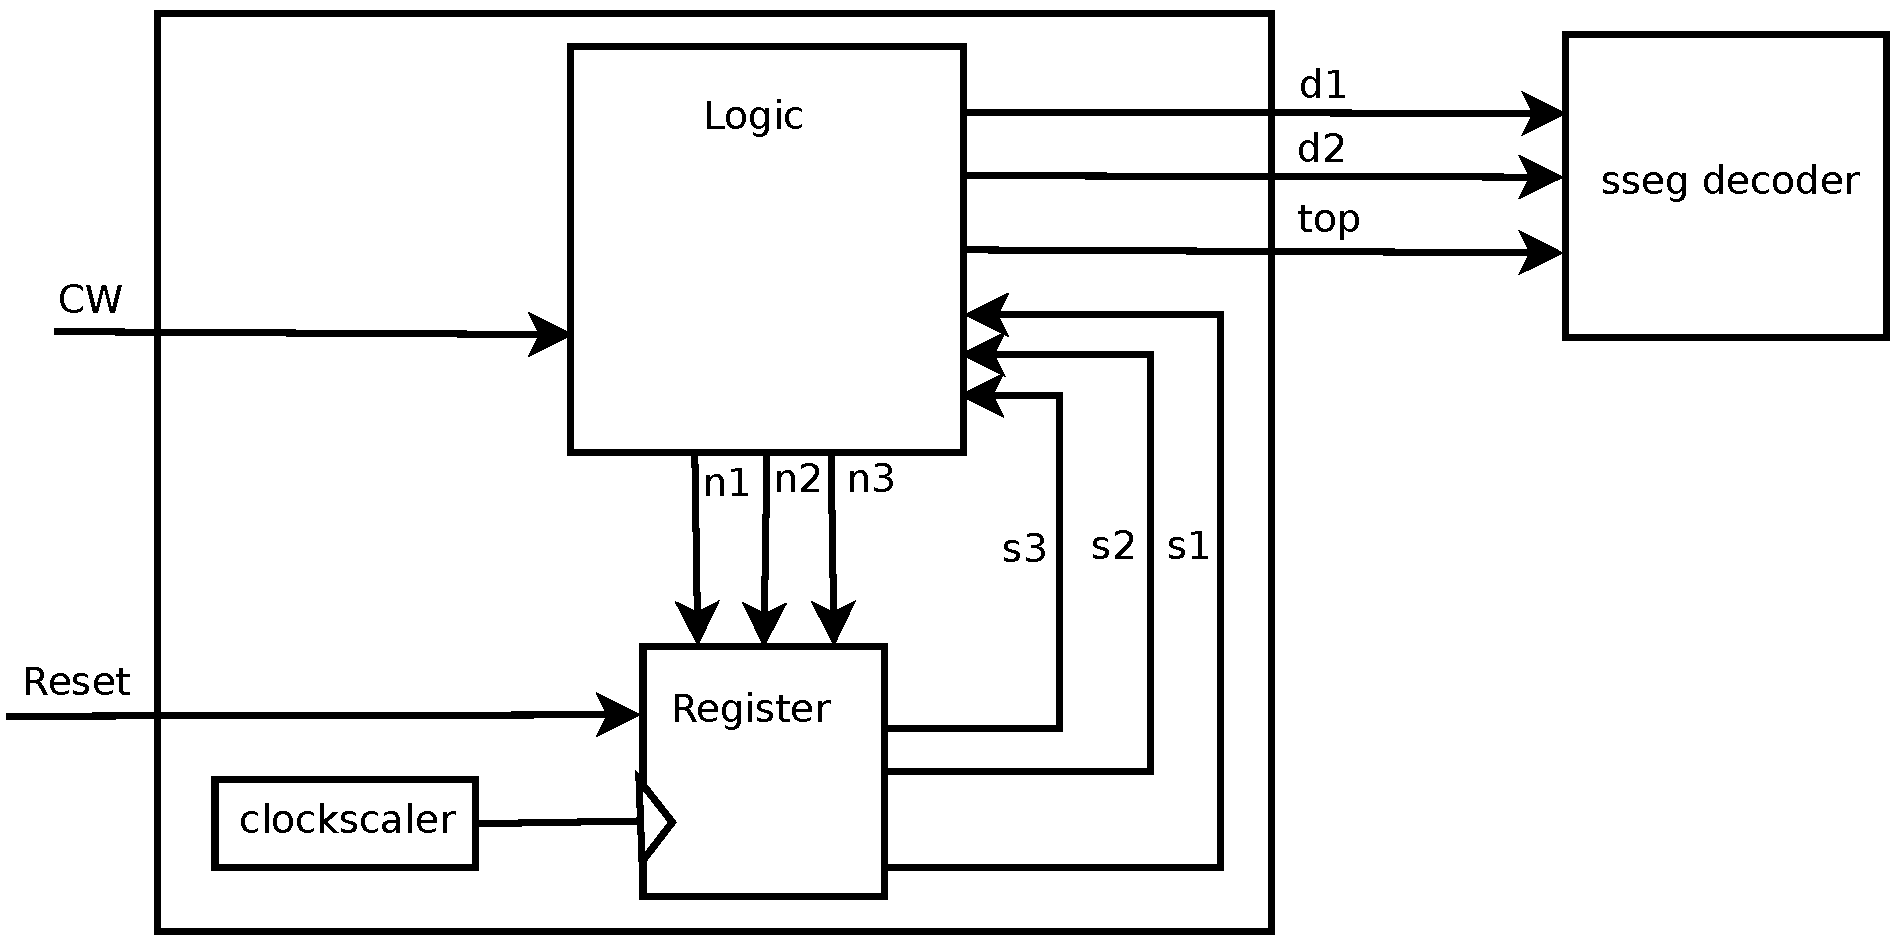
\includegraphics[height=0.4\textwidth]{fig/Block_diagram_implementation.pdf}
	\caption{Block diagram of implementation}
	\label{fig:block_diagram_implementation} 
\end{figure}
For making this implementation we have created two new VHDL modules: ``sseg\_decoder.vhd'' and ``clockscaler.vhd''. The clockscaler does a downscaling by a factor $10^{6}$ effectively setting the frequency to 5Hz (when having a period of 20ns).\\
The seven segment decoder translates inputs to the physical display.

\subsection{RTL level design}
The RTL level design was created using two muxes instead of combinatorial circuits. The code can be found in ``RTL/Runner\_logic.vhd''.